% Options for packages loaded elsewhere
\PassOptionsToPackage{unicode}{hyperref}
\PassOptionsToPackage{hyphens}{url}
%
\documentclass[
]{article}
\usepackage{amsmath,amssymb}
\usepackage{lmodern}
\usepackage{iftex}
\ifPDFTeX
  \usepackage[T1]{fontenc}
  \usepackage[utf8]{inputenc}
  \usepackage{textcomp} % provide euro and other symbols
\else % if luatex or xetex
  \usepackage{unicode-math}
  \defaultfontfeatures{Scale=MatchLowercase}
  \defaultfontfeatures[\rmfamily]{Ligatures=TeX,Scale=1}
\fi
% Use upquote if available, for straight quotes in verbatim environments
\IfFileExists{upquote.sty}{\usepackage{upquote}}{}
\IfFileExists{microtype.sty}{% use microtype if available
  \usepackage[]{microtype}
  \UseMicrotypeSet[protrusion]{basicmath} % disable protrusion for tt fonts
}{}
\makeatletter
\@ifundefined{KOMAClassName}{% if non-KOMA class
  \IfFileExists{parskip.sty}{%
    \usepackage{parskip}
  }{% else
    \setlength{\parindent}{0pt}
    \setlength{\parskip}{6pt plus 2pt minus 1pt}}
}{% if KOMA class
  \KOMAoptions{parskip=half}}
\makeatother
\usepackage{xcolor}
\usepackage[margin=1in]{geometry}
\usepackage{longtable,booktabs,array}
\usepackage{calc} % for calculating minipage widths
% Correct order of tables after \paragraph or \subparagraph
\usepackage{etoolbox}
\makeatletter
\patchcmd\longtable{\par}{\if@noskipsec\mbox{}\fi\par}{}{}
\makeatother
% Allow footnotes in longtable head/foot
\IfFileExists{footnotehyper.sty}{\usepackage{footnotehyper}}{\usepackage{footnote}}
\makesavenoteenv{longtable}
\usepackage{graphicx}
\makeatletter
\def\maxwidth{\ifdim\Gin@nat@width>\linewidth\linewidth\else\Gin@nat@width\fi}
\def\maxheight{\ifdim\Gin@nat@height>\textheight\textheight\else\Gin@nat@height\fi}
\makeatother
% Scale images if necessary, so that they will not overflow the page
% margins by default, and it is still possible to overwrite the defaults
% using explicit options in \includegraphics[width, height, ...]{}
\setkeys{Gin}{width=\maxwidth,height=\maxheight,keepaspectratio}
% Set default figure placement to htbp
\makeatletter
\def\fps@figure{htbp}
\makeatother
\setlength{\emergencystretch}{3em} % prevent overfull lines
\providecommand{\tightlist}{%
  \setlength{\itemsep}{0pt}\setlength{\parskip}{0pt}}
\setcounter{secnumdepth}{-\maxdimen} % remove section numbering
\ifLuaTeX
  \usepackage{selnolig}  % disable illegal ligatures
\fi
\IfFileExists{bookmark.sty}{\usepackage{bookmark}}{\usepackage{hyperref}}
\IfFileExists{xurl.sty}{\usepackage{xurl}}{} % add URL line breaks if available
\urlstyle{same} % disable monospaced font for URLs
\hypersetup{
  pdftitle={Implementation of Sublinear Clustering Algorithm (Rough Draft)},
  pdfauthor={James Camacho and Joseph Camacho},
  hidelinks,
  pdfcreator={LaTeX via pandoc}}

\title{Implementation of Sublinear Clustering Algorithm (Rough Draft)}
\author{James Camacho and Joseph Camacho}
\date{December 12, 2022}

\begin{document}
\maketitle

\hypertarget{implementation-of-sublinear-clustering-algorithm-rough-draft}{%
\section{Implementation of Sublinear Clustering Algorithm (Rough
Draft)}\label{implementation-of-sublinear-clustering-algorithm-rough-draft}}

\hypertarget{by-james-camacho-and-joseph-camacho}{%
\subsection{By James Camacho and Joseph
Camacho}\label{by-james-camacho-and-joseph-camacho}}

\hypertarget{overview}{%
\subsubsection{Overview}\label{overview}}

We implement the algorithm
\href{https://doi.org/10.48550/arxiv.2109.14528}{"Sublinear Time and
Space Algorithms for Correlation Clustering via Sparse-Dense
Decompositions"} by Sepehr Assadi and Chen Wang. This clusters data in a
(+/-)-labeled graph, where pluses mean two vertices are correlated and
minuses mean anticorrelation. For example, a graph of all English words
could have pluses between synonyms and minuses between antonyms. In
other datasets, such as document clustering, these graphs can be
incredibly large and dense, leading to a superlinear number of edges
compared to the vertices. Even a single pass through the edges can be
infeasible. This algorithm presents an approximation scheme that is
{\(\overset{\sim}{O}(n)\)} in the number of vertices, often sublinear in
the size of the dataset.

It requires access to the plus-labeled edges in an adjacency list, and
works as follows:

\begin{enumerate}
\tightlist
\item
  Sample a constant number of edges from each vertex.
\item
  Choose a random (sublinear) number of vertices and query every edge of
  these vertices.
\item
  Filter these vertices using the sampled edges from step one to find
  the densest ones.
\item
  Create candidates for the clusters based on the dense vertices and
  their neighbors.
\item
  Find approximate clusters from the candidates.
\end{enumerate}

If the constants are chosen right, there should be a high probability
that the candidate clusters in step four form a laminar group, i.e. each
candidate is either disjoint or a subset to any other candidate. Then,
step five consists of assigning each vertex to the largest candidate
it\textquotesingle s contained in. If it isn\textquotesingle t contained
in any candidate clusters, it is assumed to be pretty isolated and
assigned to its own cluster.

We can define a cost for the clustering-\/-\/-each time two vertices are
put in different clusters but have a plus-edge between them, the cost is
increased by one. Similarly if two vertices share a minus-edge but get
put in the same cluster, the cost increases by one. It turns out the
minus-edges are not too relevant, as two vertices with a minus-edge
should only be clustered together if they share a lot of neighbors in
the plus-subgraph, in which case the cost would increase whether or not
they get clustered together. So, by only using the plus-subgraph, it is
possible to determine good clusters with an {\(O(1)\)} approximation to
the optimum.

The accuracy of the algorithm depends on the details. How many edges do
you sample from each vertex? What is the probability you sample all the
edges for a particular vertex? What bounds do you use to filter dense
vertices?

The paper suggests sampling {\(t = O(\varepsilon^{- 2}\log n)\)}
vertices for some constant {\(\varepsilon\)}. This {\(\varepsilon\)} is
never specified in the paper, but certain theoretical results of theirs
require that {\(\varepsilon < 1/360\)}.

In step two, a vertex {\(v\)} is chosen with probability
{\(O(\log n/\deg(v))\)}. Note that this rewards sparser vertices---in a
complete graph with {\(n\)} vertices you would only expect
{\(O(\log n)\)} vertices, and thus {\(O(n\log n)\)} edges to be sampled,
while a tree would have nearly every vertex chosen. Overall, steps one
and two only require us to sample
{\(\overset{\sim}{O}(n\varepsilon^{- 2})\)} edges.

The filtering in step three is a little more complicated. First, all
vertices that have much denser neighbors should be filtered out. This is
according to the formula
{\[\varepsilon\deg(v) < |\{ u\text{~neighbors~}v:\deg(u) > (1 + \varepsilon)\deg(v)\}|.\]}Then,
sparse vertices are filtered out. Call the \emph{low} neighbors of
{\(v\)} the vertices {\(u\)} where
{\[\deg(u) < (1 + 7\varepsilon)\deg(v).\]}A low neighbor {\(u\)} is
\emph{isolated} if
{\[|\text{sampled\ neighbors}(u) \cap \text{low}(v)| < (1 - 4\varepsilon)t,\]}i.e.
very few of its neighbors are also low neighbors of {\(v\)}. If a large
fraction, at least {\(2\varepsilon\deg(v)\)}, of the low neighbors of
{\(v\)} are isolated, then {\(v\)} is considered sparse.
We\textquotesingle re left with only the densest vertices from our
sample in step two.

From here, we use some more magic numbers to build candidate clusters.
For each dense vertex {\(v\)}, we build a candidate set, including a low
neighbor {\(u\)} if
{\[1 + 22\varepsilon > \frac{\deg(u)}{\deg(v)} > \frac{(1 - 67\varepsilon)t}{|\text{sampled\ neighbors}(u) \cap \text{low}(v)|}.\]}Recall
that there are {\(t\)} sampled neighbors of {\(u\)}, so the right
inequality means that most neighbors of {\(u\)} are also low neighbors
of {\(v\)}. In most of our analysis we have {\(\varepsilon > 1/67\)}, so
this inequality doesn\textquotesingle t do much, but it will serve to
increase accuracy as {\(\varepsilon\)} gets very small.

In this paper we explore more how the choice of {\(\varepsilon\)} and
constant multiplier in {\(t = O(\varepsilon^{- 2}\log n)\)} affect the
operation count and accuracy of the algorithm. We answer questions like,
exactly how close are the candidate clusters to a laminar set family?
How many intersections can we expect? Do we \emph{really} need
{\(\varepsilon < 1/360\)} in practice, or would larger values like
{\(\varepsilon = 1/64\)}, {\(\varepsilon = 1/2\)} or
{\(\varepsilon \approx 1\)} fare equally well? How do sparser or denser
datasets change these results?

\hypertarget{choice-of-varepsilon}{%
\subsection{\texorpdfstring{Choice of
{\(\varepsilon\)}}{Choice of \textbackslash varepsilon}}\label{choice-of-varepsilon}}

Assadi and Wang\textquotesingle s main result is that their algorithm
results in a constant-approximation of the optimal clustering in
sublinear time. However, the quality of this constant depends very much
on their choice of {\(\varepsilon\)}. In particular, they showed that
the constant is roughly proportional to {\(\varepsilon^{- 2}\)}. This
makes restricting {\(\varepsilon\)} to less than {\(1/360\)} (as certain
theoretical results of theirs require) suboptimal: If the optimal
clustering of a graph has a single incorrect correllation, using their
clustering algorithm with {\(\varepsilon = 1/361\)} could have on the
order of over 100,000 incorrect edges. This is a terrible approximation!

Luckily, in practice {\(\varepsilon\)} can be raised to much larger
values while maintaining sublinear time in edges, vastly improving the
approximation of the clustering. In order to test this, we use two
datasets. The first is a graph of English words with plus-edges between
synonyms and minus-edges between antonyms. The second is a random graph
with ten thousand vertices, one million edges, and ten clusters; edges
within a cluster are assigned a plus while edges between clusters are
labelled with a minus, however we randomly flip between 10\% and 45\% of
these correlations.

For both datasets running time improved as {\(\varepsilon\)} increased,
as fewer edges needed to be considered. However, the thesaurus dataset
differed from the random dataset with the errors. As {\(\varepsilon\)}
transitioned from less than {\(0.25\)} to more than {\(0.25\)} we saw a
pronounced increase in the number of errors on the real-world data,
while a marked improvement in accurracy for the random dataset. Note
that determining the optimum for the thesaurus dataset is NP-hard, so we
instead give the error count.

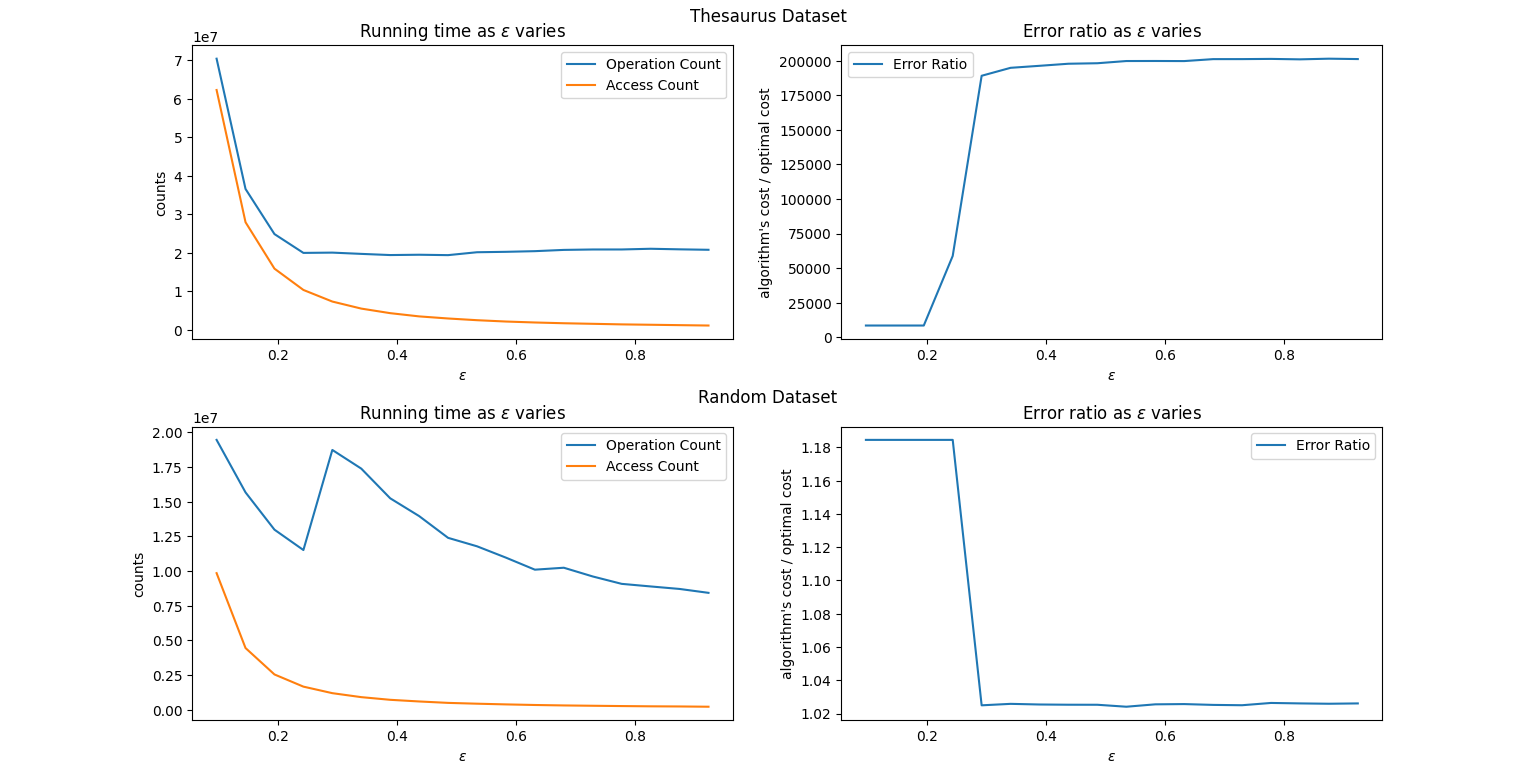
\includegraphics{images/opposite_trends.png}\\
This difference likely arises as there are only \textasciitilde8,000
antonyms compared to \textasciitilde200,000 synonyms in the thesaurus.
Putting all words into one cluster is guaranteed to have very few
errors, while separating into multiple clusters risks synonyms being in
different clusters.

For the random dataset, we see this rapid improvement at
{\(\varepsilon = 0.25\)} even as we change the fraction of edge
correlations that are flipped, how many clusters there are, or the size
of the graph. For example, the below graphs show the algorithm run with
{\(\varepsilon < 0.25\)} and {\(\varepsilon > 0.25\)} and a varying
number of edges. Even with very few edges we have over four times the
error when {\(\varepsilon < 0.25\)}, and as it gets denser this
increases to over twenty times!

\begin{longtable}[]{@{}cc@{}}
\toprule()
{\(\varepsilon < 0.25\)} & {\(\varepsilon > 0.25\)} \\
\midrule()
\endhead
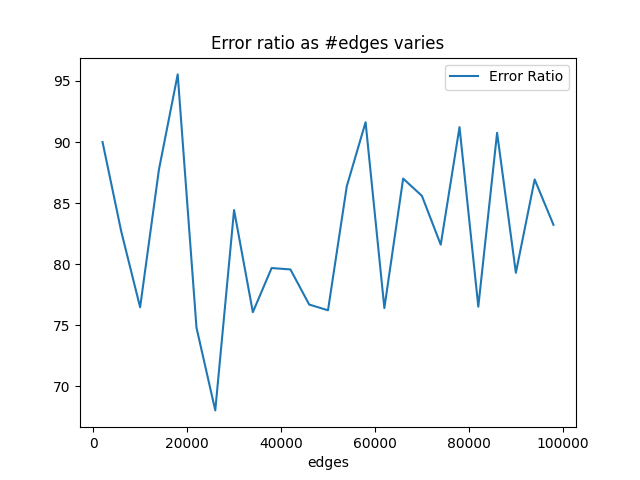
\includegraphics{images/error_ratio_as_edges_varies_low_epsilon.png}
&
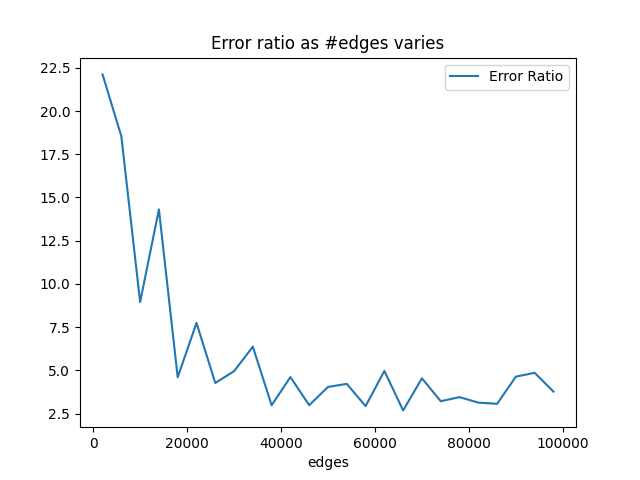
\includegraphics{images/error_ratio_as_edges_varies_high_epsilon.png} \\
\bottomrule()
\end{longtable}

To get a denser model based on real-world data, we create a new dataset
using word vectors. It is well known their dot products are a measure of
correlation, with very positive dot products being highly correlated
while negative dot products are anticorrelated, so we assign plus-edges
to the top percentiles of these dot products, and minus-edges to the
bottom. Changing this fraction allows for sparser or denser graphs.

For all levels of sparsity, we see an error trend similar to that of the
random graphs:\\
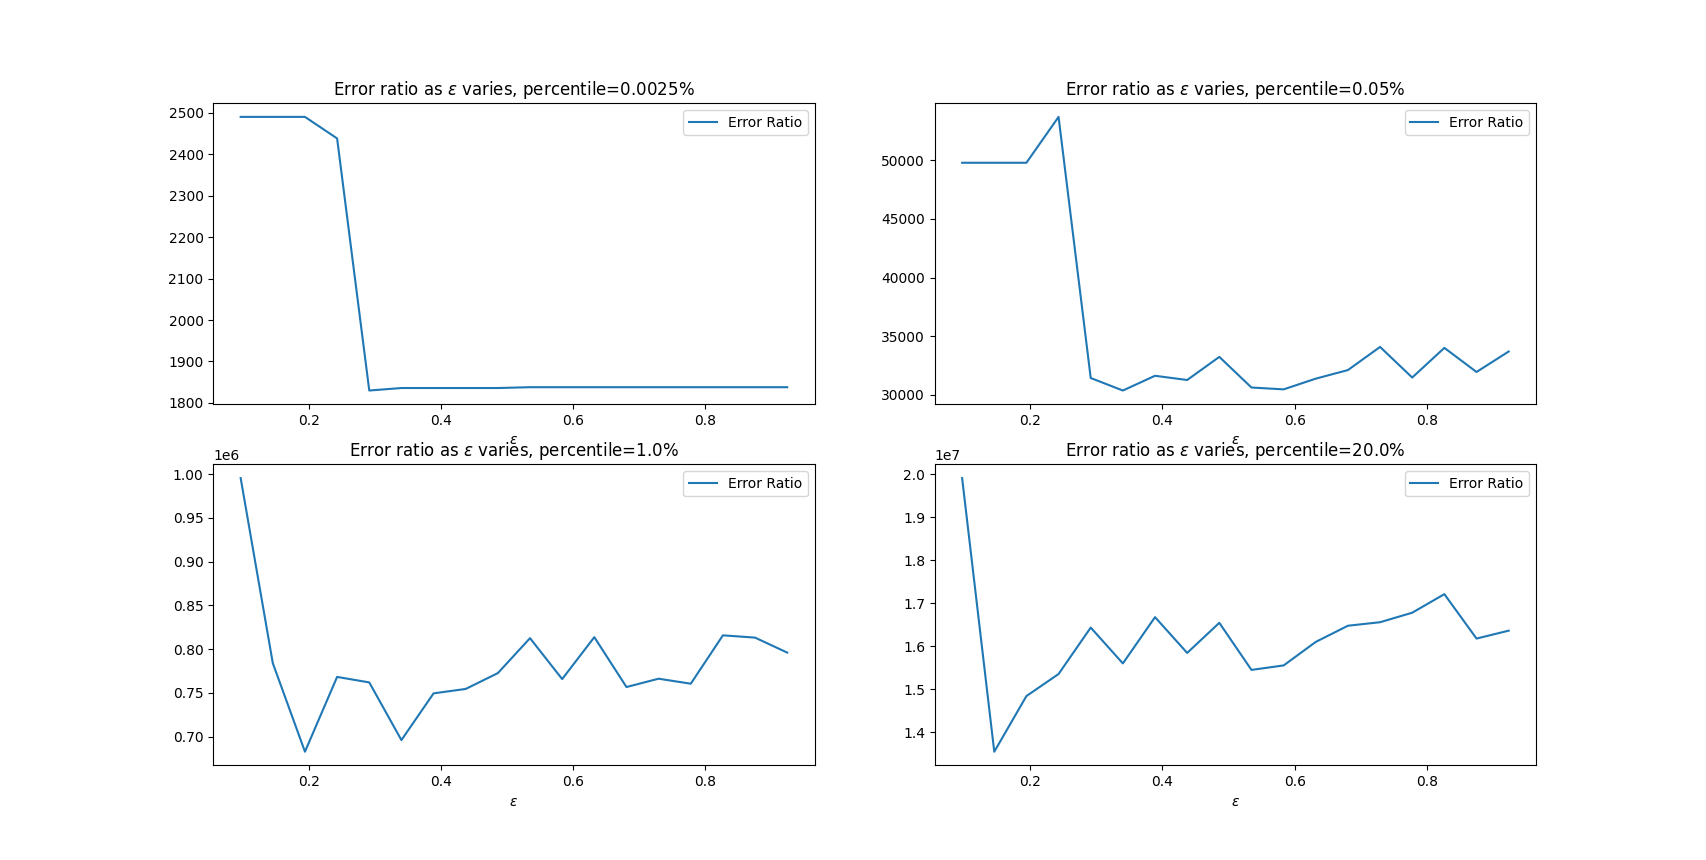
\includegraphics{images/percentile_change.png}\\
For both the random graph and the graph based on word vectors, the best
clustering occurs when {\(\varepsilon\)} is slightly larger than
{\(0.25\)}.

Likewise, the running time improves as {\(\varepsilon\)} increases:\\
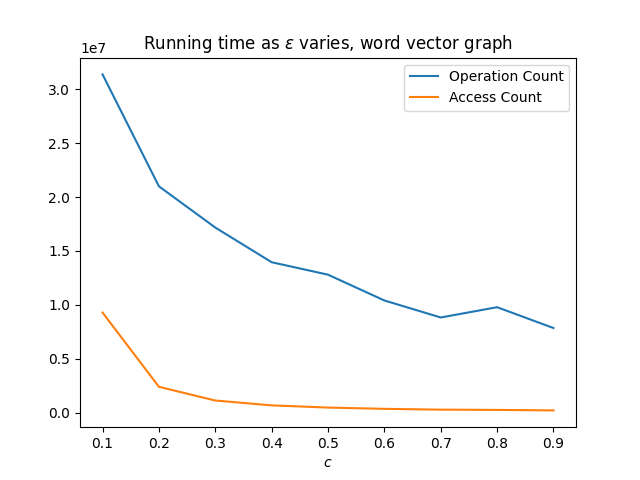
\includegraphics{images/running_time_as_eps_varies_word_vector.png}

This suggests several things, most notably that filtering by isolated
neighbors is actually detrimental to the performance of the algorithm!
Although it\textquotesingle s theoretically necessary to do this
filtering to gurantee an {\(O(1)\)} approximation (as the thesaurus
dataset somewhat shows), in practice it\textquotesingle s not only
faster to not do so, but also more accurate.

In conclusion, real world data often looks similar to the random dataset
we built, and for these types of data, setting {\(\varepsilon\)} to be
slightly more than {\(0.25\)} is a good choice.

\hypertarget{choice-of-c}{%
\subsection{\texorpdfstring{Choice of
{\(c\)}}{Choice of c}}\label{choice-of-c}}

In their paper, Assadi and Wang state that "there is an absolute
constant {\(c > 0\)}" for which their algorithm works, but they never
specify exactly what {\(c\)} has to be. In fact, they only imply what
restrictions {\(c\)} might have by constraints on other variables. These
constraints imply that {\(c\)} to be on the order of at least
{\(\varepsilon^{2}\)}. Since {\(\varepsilon^{2}\)} is rather small, this
means that {\(c\)} can be just about anything.

Nevertheless, setting {\(c = \varepsilon^{2}\)} is hardly useful. While
lowering {\(c\)} speeds up the algorithm by requiring fewer graph
accesses, it also lowers its performance because the algorithm has less
information to make use of. In this section, we explore the tradeoffs of
what {\(c\)} should be, and demonstrate that {\(c \approx 2\)} yields
good results with competitive results.

In the previous section, we showed that a good choice of
{\(\varepsilon\)} is not much more than {\(0.25\)}. For this section, we
set {\(\varepsilon = 0.3\)}.

Using the random graph, we get the following approximations as {\(c\)}
varies:\\
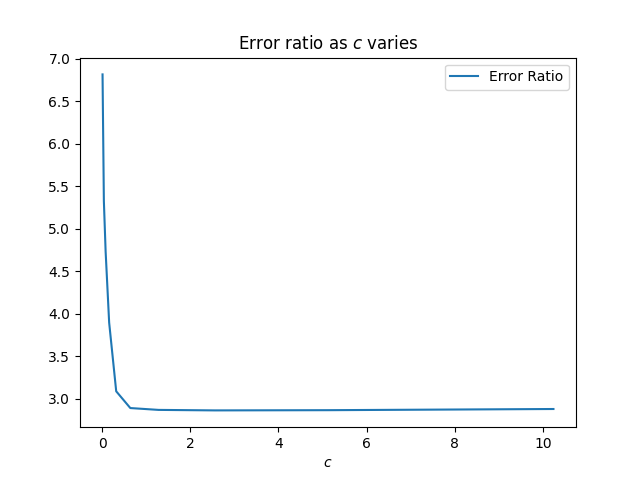
\includegraphics{images/error_ratio_as_c_varies.png}\\
Using the word vector graph gives a similar chart:\\
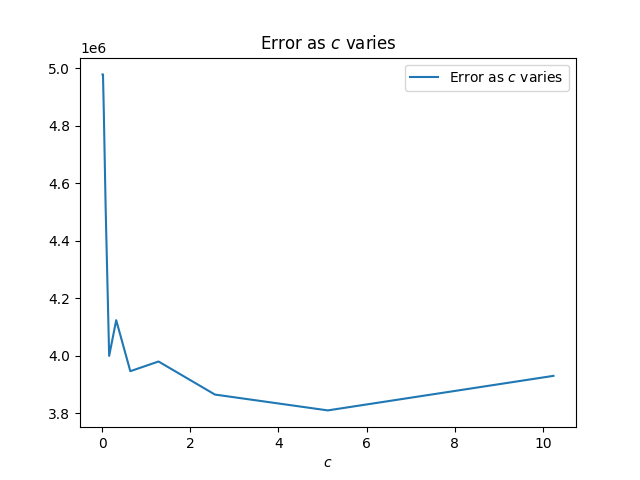
\includegraphics{images/error_ratio_as_c_varies_word_vector.png}

In both cases, the running time scales linearly with {\(c\)}:

\begin{longtable}[]{@{}cc@{}}
\toprule()
Random & Word Vector \\
\midrule()
\endhead
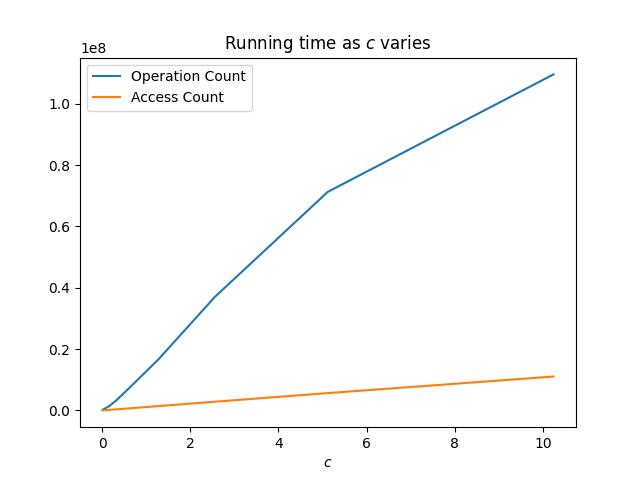
\includegraphics{images/running_time_as_c_varies.png}
&
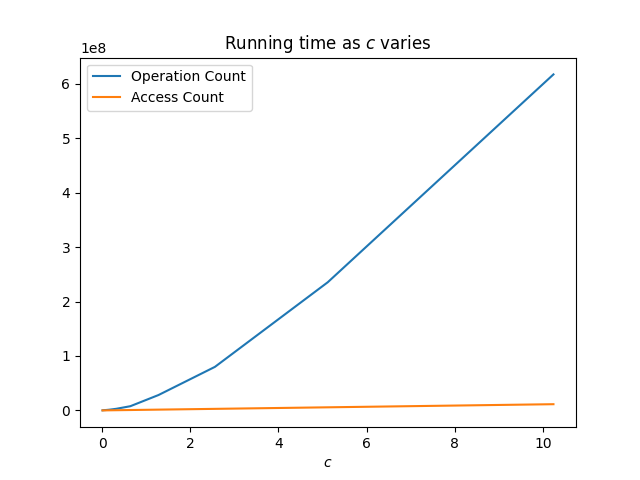
\includegraphics{images/running_time_as_c_varies_word_vector.png} \\
\bottomrule()
\end{longtable}

A good trade off, then, between runtime and error ratio appears to be
setting {\(c \approx 2\)}.

\hypertarget{sublinear-time}{%
\subsection{Sublinear Time}\label{sublinear-time}}

It\textquotesingle s easy enough to theoretically show that the
algorithm described above is sublinear in the number of edges no matter
what the specific choices of {\(\varepsilon\)} and {\(c\)} are. (Indeed,
Assadi and Wang\textquotesingle s paper is important not because their
algorithm is sublinear in time, but because it has {\(O(1)\)}
competitiveness.) In this section, we demonstrate this by analyzing the
runtime for fixed {\(\varepsilon = 0.3\)} and {\(c = 2\)}.

TODO: Uh oh James! This doesn\textquotesingle t actually work! The
graphs appear to have linear time!!!\\
Random \textbar{} Word Vector\\
:-\/-\/-\/-:\textbar:-\/-\/-\/-:\\
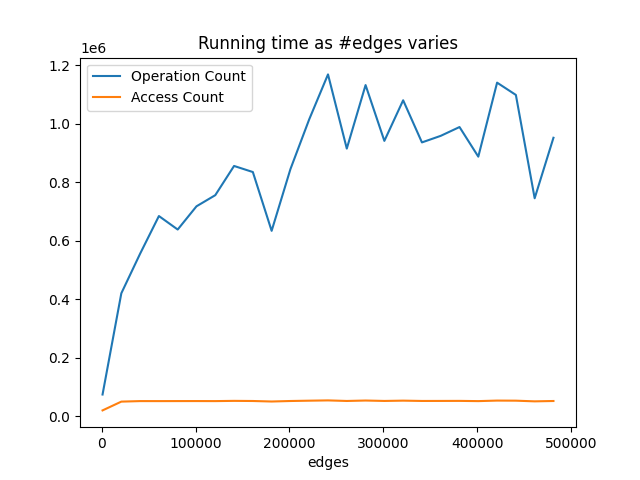
\includegraphics{images/running_time_as_edges_varies.png}
\textbar{}
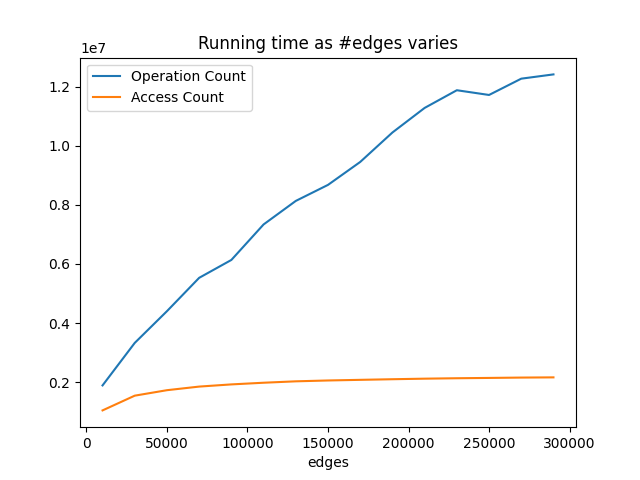
\includegraphics{images/running_time_as_edges_varies_word_vector.png}

I think this is where we need the filter part! We have sublinear time
for low {\(\varepsilon\)}. The following graph is for where
{\(\varepsilon = 0.01\)}:\\
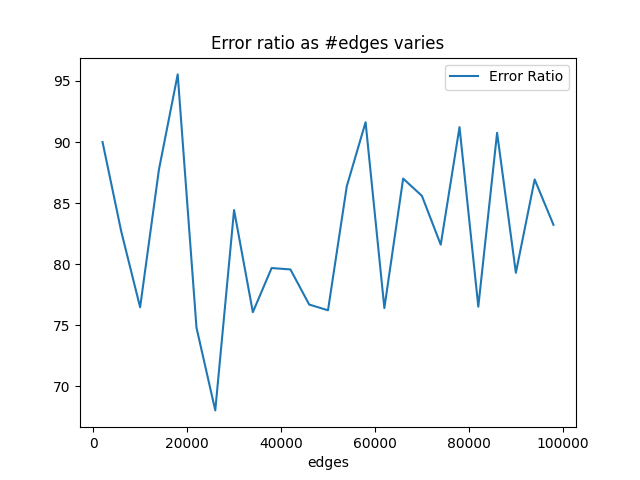
\includegraphics{images/error_ratio_as_edges_varies_low_epsilon.png}

\hypertarget{laminar-candidate-clusters}{%
\subsection{Laminar Candidate
Clusters}\label{laminar-candidate-clusters}}

Assadi and Wang make the claim that the candidate clusters have a high
probability of forming a laminar set family. Every pair of candidates
should either be disjoint, or one is a subset of the other. Suppose two
candidates do not satisfy this laminar property. Their symmetric
difference is all elements contained in exactly one subset but not the
other, and so the sum of the symmetric differences is a measure of how
far off from laminar the candidates are. Normalizing by number of
vertices and number of candidate sets gives the following graphs:

\textbf{Random graph,}
{\(V = 10^{4},E = 10^{6},\text{clusters} = 10,\text{flip} = 10\%\)}.\\
{\(c = 2\)} is fixed, {\(\varepsilon\)} varies. \textbar{}
{\(\varepsilon = 0.3\)} is fixed, {\(c\)} varies.\\
:-\/-\/-\/-:\textbar:-\/-\/-\/-:\\
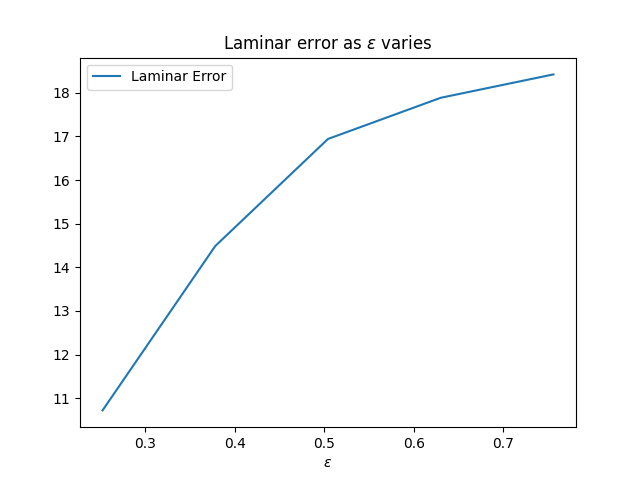
\includegraphics{images/laminar_error_as_epsilon_varies.png}
\textbar{}
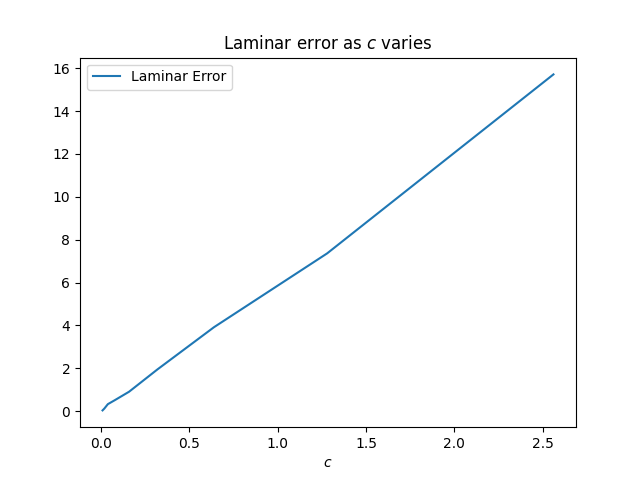
\includegraphics{images/laminar_error_as_c_varies.png}

\textbf{Word vector graph,} {\(V = 10^{4},E = 5\%\)}.\\
{\(c = 2\)} is fixed, {\(\varepsilon\)} varies. \textbar{}
{\(\varepsilon = 0.3\)} is fixed, {\(c\)} varies.\\
:-\/-\/-\/-:\textbar:-\/-\/-\/-:\\
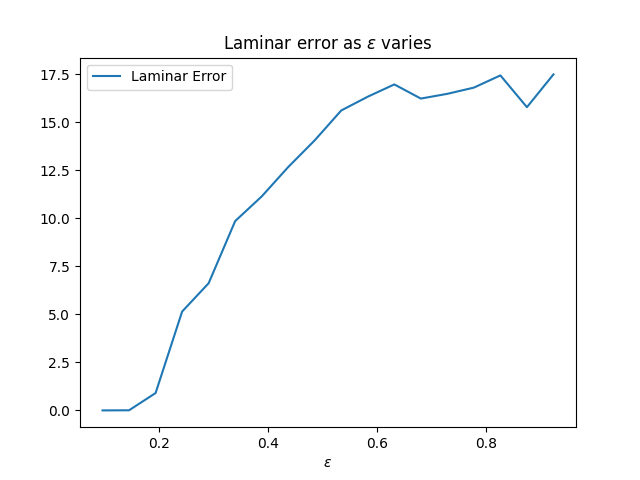
\includegraphics{images/laminar_error_as_epsilon_varies_word_vector.png}
\textbar{}
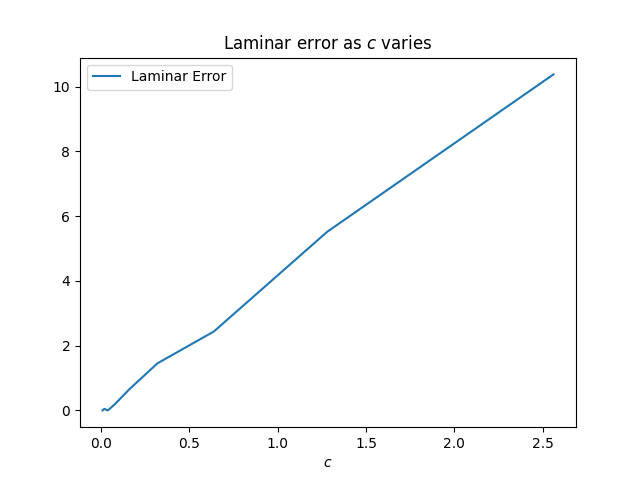
\includegraphics{images/laminar_error_as_c_varies_word_vector.png}\\
When {\(\varepsilon\)} is very small there are no candidates, but
otherwise we see a linear increase in laminar error as {\(c\)}
increases, and approximately sublinear for {\(\varepsilon\)}. From our
earlier analysis, for graphs of this size we want
{\(\varepsilon \approx 0.3\)} and {\(c \approx 2\)}, which would give
the average vertex at most ten potential clusters, around {\(1\%\)} of
the total number of clusters. This is pretty good. It would be
interesting for a future paper to explore a recursive strategy using
these candidate clusters, instead of just assigning vertices through a
loop of the largest candidates.

\hypertarget{conclusion}{%
\subsection{Conclusion}\label{conclusion}}

In this paper, we implemented Sepehr Assadi and Chen
Wang\textquotesingle s algorithm for correlation clustering and
empirically showed that their theoretical results held true.

\hypertarget{references}{%
\subsection{References}\label{references}}

\href{https://doi.org/10.48550/arxiv.2109.14528}{"Sublinear Time and
Space Algorithms for Correlation Clustering via Sparse-Dense
Decompositions"}

\end{document}
